\section{Invasion Percolation for Search Diversification}
We adapt the BIP model as an exploration mechanism for best-first search.
%% doesnt look so important --- pretty obvious
% The basic idea is: Given a search graph that we would like to search in an unbiased manner,
% we treat it as a graph with randomly assigned edge costs and apply BIP.
Previous work on BIP was on physical simulations with relatively small graphs, 
and to our knowledge, this is the first application of BIP  to complex \emph{implicit} graphs.
% The original mapping from BIP to an equivalent graph algorithm (Prim's method) assumes an explicit representation of the graph. 
% Here, we adapt their method for the implicit graphs which are searched using BFS.


The actual implementation of BIP is quite simple:
%It can be implemented as
A % pseudo heuristic % in this case, just calling $\bip$ a ``function'' seems sufficient -- no need to invent new term
function $\bip$ returns a randomly selected value 
for each search edge that caused the node to be evaluated.
%It is important to note that this random value must be memoized, i.e.,
For each edge, the function should always return the same value  once a random value is assigned to that edge. This requires storage whose size is linear in the number of edges that are explored.
% While it is possible to avoid this storage with a random hash function such as Zobrist hash \cite{zobrist1970new}, the preliminary experiment showed that it incurs the additional cost of node evaluation. Therefore, we simply generate a new value by a pseudo random number generator.

% While a naive implementation assigns a random value to  an operator / search node pair, this results in much larger memory
% usage and also incurs more search overhead per node (e.g., instantiating a pair, increased cost of retrieving the
% memoized value from the cache). Thus, in our implementation, we assign a random integer value to a search
% node and to an operator separately, then take the XOR of the values.

For intra-plateau exploration, $\bip$ is used to break ties in a plateau induced by the primary heuristic function $h$, i.e. $[h,\bip,*]$.
Since nodes are sorted in increasing order of the memoized random value attached to each edge, the node expansion order within a plateau follows that of Prim's method.
For inter-plateau exploration, we alternate the expansion between standard GBFS and a queue sorted by $\bip$: $\mit{alt}([h],[\bip])$, just as in Type-GBFS.


%moving this after the ``IP for diversification'' heading because this text mentions search and expansions
Consider applying BIP to the DAG in \refig{fig:model}.
There is a non-negligible probability that the search finds the solution without expanding high-b branch (\refig{fig:ip-success}):
This occurs when the value $v(H_1)$ of $H_1$ is higher than the value of any of $L_1\ldots L_4$,
whose probability is 1/5
 (follows from $\int_0^1 dv(H_1) Pr(\forall i; v(L_i)\leq v(H_1)) = \int_0^1 x^4dx$). 
In this case, node $H_1$ is acting as an embankment, causing nodes in the  low-b branch to be expanded.
In contrast, the opposite case is very unlikely:
$L_1$ \emph{could} be expanded after expanding all of $H_{d,b}$ for $1\leq d\leq 4$ and $1\leq b \leq B$,
 but the probability of this,  $1/(2B+3)$,  is very small (assuming large $B$).

\begin{figure}[htb]
 \centering
 % 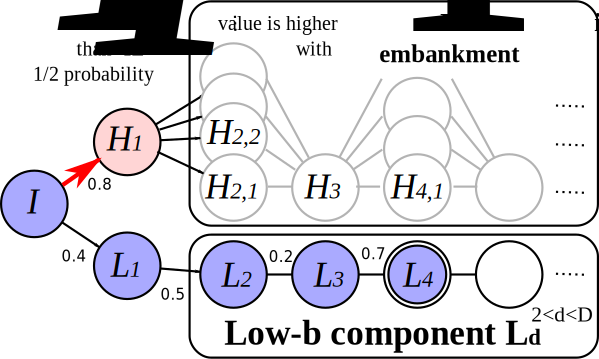
\includegraphics[width=0.8\linewidth]{img/model/bip1-1.pdf}
 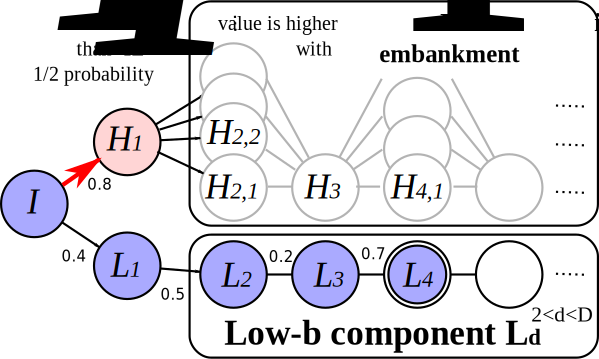
\includegraphics[width=0.49\linewidth]{img/model/bip1-1.pdf}
 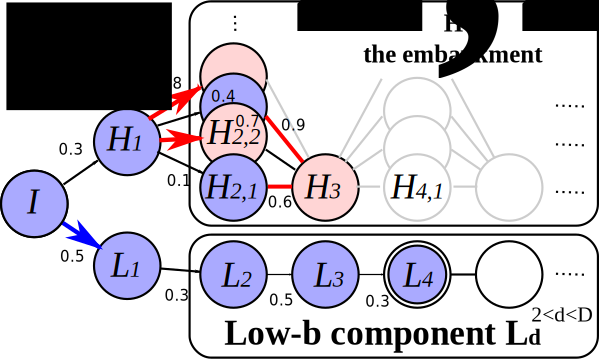
\includegraphics[width=0.49\linewidth]{img/model/bip2-1.pdf}
 \caption{Examples where BIP successfully prevents the expansion of high-B branch.}
 \label{fig:ip-success}
\end{figure}

Also consider the case when $H_1$ is expanded with probability $4/5$.
Even if this embankment is broken, $H_3$ could act as another embankment again with probability $1/5$.
Moreover, it also avoids expanding large number of nodes in $H_{2,i}$ whose values are higher than $L_1\ldots L_4$.
$B/5$ of the nodes are not expanded on average because each node is not expanded with the same probability $1/5$.

Thus, at every possible ``bottleneck'' in the search space that forms an embankment, BIP tends to start looking at the other branches.
Since this is affected by the least width of a subgraph rather than the maximum,
it is less likely to suffer from the pathological behavior exemplified by \refig{fig:model}.

% This shape is known as a random fractal whose Hausdorff dimension is less than the space dimension.

Node expansion order according to $\bip$ differs  significantly from that of \ro (pure random selection).
% 
\ro is equivalent to performing a random sort and select the first node, i.e., \ro essentially assigns a \emph{new} random value to \emph{all} nodes at every single expansion.
In contrast, $\bip$ assigns a value to each edge only once, which develops embankments and allows unexplored ``holes'' to have longer lifetimes.
% 
% In $\bip$, once a hole is surrounded by high-valued edges, it keeps being unexplored until all low-valued edges are traversed. This embankment prevents exploration into the hole and is critical to forming a fractal structure.
% 
Consider what would happen if we switch the behavior from $\bip$ to \ro starting from the state shown in \refig{fig:ip}. Since all nodes are assigned a new random value at each expansion, the embankment nodes are more likely to be expanded, filling the holes more quickly. Thus, running \ro results in a more solid, denser expansion biased to the left, near the initial nodes.





There is one difference between the assumptions made by BIP/Prim \cite{barabasi1996invasion} and classical planning.
The search spaces of classical planning are directed while BIP/Prim assumes undirected graphs. Thus, although Prim's method finds the minimum spanning tree on an undirected graph, it may not return the minimum-weight tree on a directed graph. This, however, does not affect the completeness of our search algorithm because it just changes the order of expansion (BIP-based search diversification does not prune any nodes).
% 
% If used as intra-plateau diversification,
% The expected quality of the solution does not change, up to tiebreaking. In order to find better solutions with GBFS, one can sort the nodes preferring smaller $g$ value for tiebreaking, i.e. $[h,g,*]$ sorting strategy, but it does not preclude us from applying $\bip$ for further tiebreaking, i.e. $[h,g,\bip,*]$. Although these are possible, in this paper we solely focus on satisficing solutions for the sake of clarity and simplicity. Evaluating the impact of such $g$-based tiebreaking scheme on the solution cost is an avenue of future work.
% 
% Finally, 
Adopting algorithms for minimum spanning arborescence for directed graphs \cite{chu1965shortest,edmonds1967optimum,tarjan1977finding,gabow1986efficient} to search diversification is a direction for future work.%. However, currently we have  no straightforward way to adopt these algorithms for diversification. (A direction for future work.)

